\newpage
\null
\thispagestyle{empty}
\newpage

\addcontentsline{toc}{chapter}{Malachi}
% Safely inserts your illustration full-bleed on its own page.
% This completely bypasses the page builder, headers, and geometry bugs!
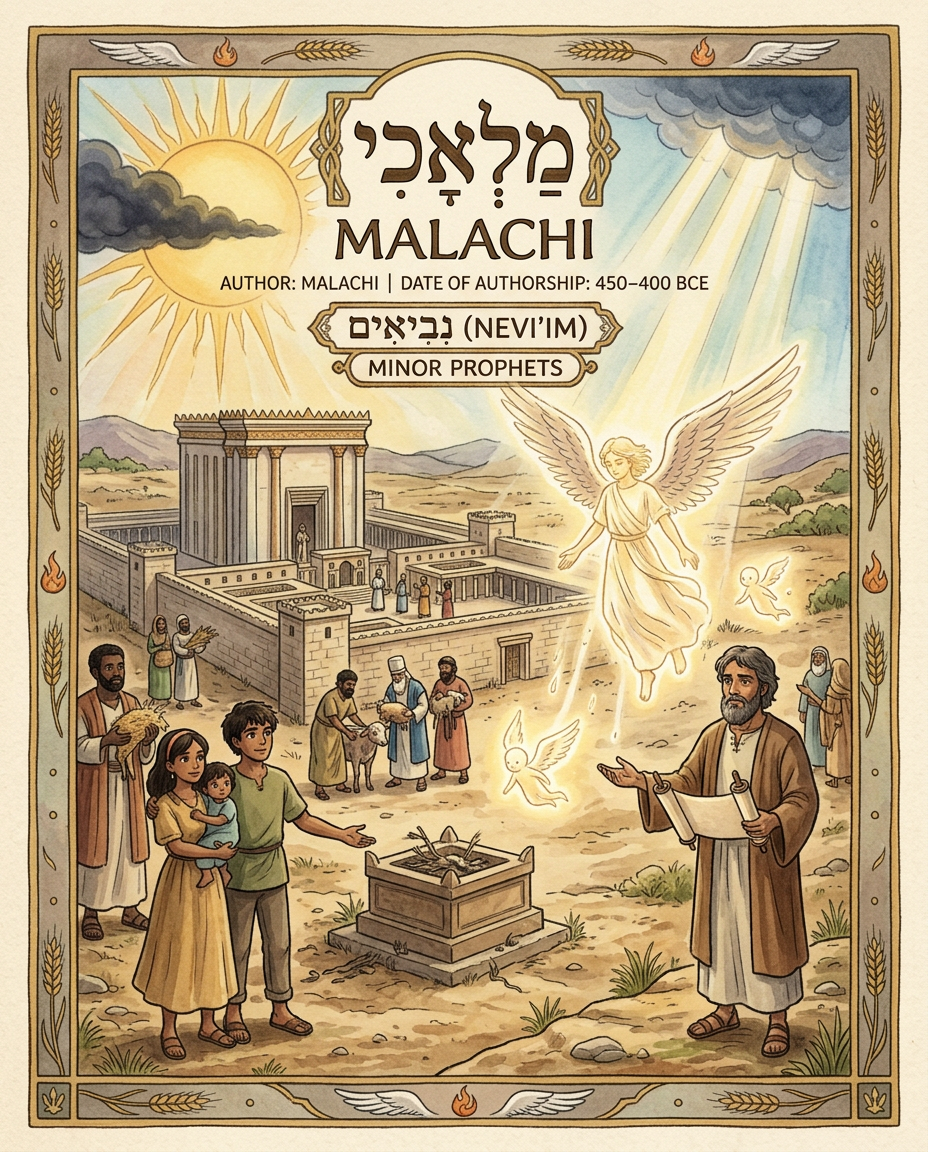
\includepdf[pages=1, fitpaper=false, width=\paperwidth, height=\paperheight, , keepaspectratio=false]{images/divider2/malachi_2.png}
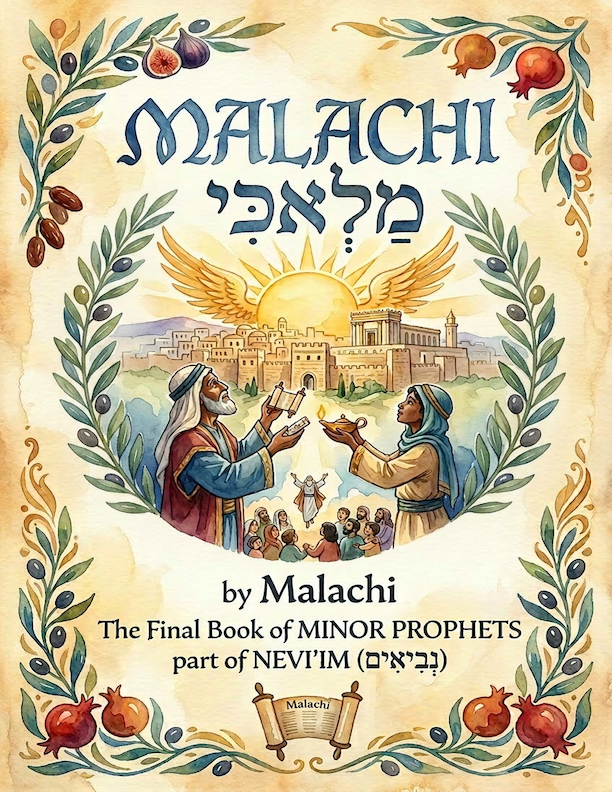
\includepdf[pages=1, fitpaper=false, width=\paperwidth, height=\paperheight, , keepaspectratio=false]{images/divider1/malachi.png}

\includepdf[pages=1, fitpaper=false, width=\paperwidth, height=\paperheight, , keepaspectratio=false]{images/8.5x11-Dot-Grid.png}

\includepdf[pages=1, fitpaper=false, width=\paperwidth, height=\paperheight, , keepaspectratio=false]{images/8.5x11-Dot-Grid.png}

\mybook{Malachi}
\vspace{-1.36in}


\mychapter{} \myverse*{}A revelation, the LORD’s\footnote{1:1 When rendered in ALL CAPITAL LETTERS, “LORD” or “GOD” is the translation of God’s Proper Name.} word to Israel by Malachi.


\myverse{}“I have loved you,” says the LORD.

Yet you say, “How have you loved us?”

“Wasn’t Esau Jacob’s brother?” says the LORD, “Yet I loved Jacob; \myverse{}but Esau I hated, and made his mountains a desolation, and gave his heritage to the jackals of the wilderness.” \myverse{}Whereas Edom says, “We are beaten down, but we will return and build the waste places,” the LORD of Hosts says, “They shall build, but I will throw down; and men will call them ‘The Wicked Land,’ even the people against whom the LORD shows wrath forever.”


\myverse{}Your eyes will see, and you will say, “The LORD is great—even beyond
the border of Israel!”


\myverse{}“A son honors his father, and a servant his master. If I am a father, then where is my honor? And if I am a master, where is the respect due me?” says the LORD of Hosts to you priests who despise my name. “You say, ‘How have we despised your name?’ \myverse{}You offer polluted bread on my altar. You say, ‘How have we polluted you?’ In that you say, ‘The LORD’s table is contemptible.’ \myverse{}When you offer the blind for sacrifice, isn’t that evil? And when you offer the lame and sick, isn’t that evil? Present it now to your governor! Will he be pleased with you? Or will he accept your person?” says the LORD of Hosts.


\myverse{}“Now, please entreat the favor of God,\footnote{1:9 The Hebrew word rendered “God” is “אֱלֹהִ֑ים” (Elohim).} that he may be gracious to us. With this, will he accept any of you?” says the LORD of Hosts.


\myverse{}“Oh that there were one among you who would shut the doors, that you might not kindle fire on my altar in vain! I have no pleasure in you,” says the LORD of Hosts, “neither will I accept an offering at your hand. \myverse{}For from the rising of the sun even to its going down, my name is great among the nations, and in every place incense will be offered to my name, and a pure offering; for my name is great among the nations,” says the LORD of Hosts. \myverse{}“But you profane it when you say, ‘The LORD’s table is polluted, and its fruit, even its food, is contemptible.’ \myverse{}You say also, ‘Behold,\footnote{1:13 “Behold”, from “הִנֵּה”, means look at, take notice, observe, see, or gaze at. It is often used as an interjection.} what a weariness it is!’ And you have sniffed at it”, says the LORD of Hosts; “and you have brought that which was taken by violence, the lame, and the sick; thus you bring the offering. Should I accept this at your hand?” says the LORD.


\myverse{}“But the deceiver is cursed who has in his flock a male, and vows and sacrifices to the Lord\footnote{1:14 The word translated “Lord” (mixed case) is “Adonai.”} a defective thing; for I am a great King,” says the LORD of Hosts, “and my name is awesome among the nations.”


% MALACHI 2
\mychapter{} \myverse*{}“Now, you priests, this commandment is for you. \myverse{}If you will not listen, and if you will not take it to heart, to give glory to my name,” says the LORD of Hosts, “then I will send the curse on you, and I will curse your blessings. Indeed, I have cursed them already, because you do not take it to heart. \myverse{}Behold, I will rebuke your offspring,\footnote{2:3 or, seed} and will spread dung on your faces, even the dung of your feasts; and you will be taken away with it. \myverse{}You will know that I have sent this commandment to you, that my covenant may be with Levi,” says the LORD of Hosts. \myverse{}“My covenant was with him of life and peace; and I gave them to him that he might be reverent toward me; and he was reverent toward me, and stood in awe of my name. \myverse{}The law of truth was in his mouth, and unrighteousness was not found in his lips. He walked with me in peace and uprightness, and turned many away from iniquity. \myverse{}For the priest’s lips should keep knowledge, and they should seek the law at his mouth; for he is the messenger of the LORD of Hosts. \myverse{}But you have turned away from the path. You have caused many to stumble in the law. You have corrupted the covenant of Levi,” says the LORD of Hosts. \myverse{}“Therefore I have also made you contemptible and wicked before all the people, according to the way you have not kept my ways, but have had respect for persons in the law. \myverse{}Don’t we all have one father? Hasn’t one God created us? Why do we deal treacherously every man against his brother, profaning the covenant of our fathers? \myverse{}Judah has dealt treacherously, and an abomination is committed in Israel and in Jerusalem; for Judah has profaned the holiness of the LORD which he loves, and has married the daughter of a foreign god. \myverse{}The LORD will cut off the man who does this, him who wakes and him who answers, out of the tents of Jacob and him who offers an offering to the LORD of Hosts.


\myverse{}“This again you do: you cover the LORD’s altar with tears, with weeping, and with sighing, because he doesn’t regard the offering any more, neither receives it with good will at your hand. \myverse{}Yet you say, ‘Why?’ Because the LORD has been witness between you and the wife of your youth, against whom you have dealt treacherously, though she is your companion and the wife of your covenant. \myverse{}Did he not make you one, although he had the residue of the Spirit? Why one? He sought godly offspring. Therefore take heed to your spirit, and let no one deal treacherously against the wife of his youth. \myverse{}One who hates and divorces”, says the LORD, the God of Israel, “covers his garment with violence!” says the LORD of Hosts. “Therefore pay attention to your spirit, that you don’t be unfaithful.


\myverse{}You have wearied the LORD with your words. Yet you say, ‘How have we wearied him?’ In that you say, ‘Everyone who does evil is good in the LORD’s sight, and he delights in them;’ or ‘Where is the God of justice?’


% MALACHI 3
\mychapter{} \myverse*{}“Behold, I send my messenger, and he will prepare the way before me! The Lord, whom you seek, will suddenly come to his temple. Behold, the messenger of the covenant, whom you desire, is coming!” says the LORD of Hosts. \myverse{}“But who can endure the day of his coming? And who will stand when he appears? For he is like a refiner’s fire, and like launderers’ soap; \myverse{}and he will sit as a refiner and purifier of silver, and he will purify the sons of Levi, and refine them as gold and silver; and they shall offer to the LORD offerings in righteousness. \myverse{}Then the offering of Judah and Jerusalem will be pleasant to the LORD as in the days of old and as in ancient years.


\myverse{}I will come near to you to judgment. I will be a swift witness against the sorcerers, against the adulterers, against the perjurers, and against those who oppress the hireling in his wages, the widow, and the fatherless, and who deprive the foreigner of justice, and don’t fear me,” says the LORD of Hosts.


\myverse{}“For I, the LORD, don’t change; therefore you, sons of Jacob, are not consumed. \myverse{}From the days of your fathers you have turned away from my ordinances and have not kept them. Return to me, and I will return to you,” says the LORD of Hosts. “But you say, ‘How shall we return?’


\myverse{}Will a man rob God? Yet you rob me! But you say, ‘How have we robbed you?’ In tithes and offerings. \myverse{}You are cursed with the curse; for you rob me, even this whole nation. \myverse{}Bring the whole tithe into the storehouse, that there may be food in my house, and test me now in this,” says the LORD of Hosts, “if I will not open you the windows of heaven, and pour you out a blessing, that there will not be enough room for. \myverse{}I will rebuke the devourer for your sakes, and he shall not destroy the fruits of your ground; neither shall your vine cast its fruit before its time in the field,” says the LORD of Hosts. \myverse{}“All nations shall call you blessed, for you will be a delightful land,” says the LORD of Hosts.


\myverse{}“Your words have been harsh against me,” says the LORD. “Yet you say, ‘What have we spoken against you?’ \myverse{}You have said, ‘It is vain to serve God,’ and ‘What profit is it that we have followed his instructions and that we have walked mournfully before the LORD of Hosts? \myverse{}Now we call the proud happy; yes, those who work wickedness are built up; yes, they tempt God, and escape.’


\myverse{}Then those who feared the LORD spoke one with another; and the LORD listened and heard, and a book of memory was written before him for those who feared the LORD and who honored his name. \myverse{}They shall be mine,” says the LORD of Hosts, “my own possession in the day that I make. I will spare them, as a man spares his own son who serves him. \myverse{}Then you shall return and discern between the righteous and the wicked, between him who serves God and him who doesn’t serve him.


% MALACHI 4
\mychapter{} \myverse*{}“For behold, the day comes, burning like a furnace, when all the proud and all who work wickedness will be stubble. The day that comes will burn them up,” says the LORD of Hosts, “so that it will leave them neither root nor branch. \myverse{}But to you who fear my name shall the sun of righteousness arise with healing in its wings. You will go out and leap like calves of the stall. \myverse{}You shall tread down the wicked; for they will be ashes under the soles of your feet in the day that I make,” says the LORD of Hosts.


\myverse{}“Remember the Torah of Moses my servant, which I commanded to him
in Horeb for all Israel, even statutes and ordinances.


\myverse{}Behold, I will send you Elijah the prophet before the great and
terrible day of the LORD comes. \myverse{}He will turn the hearts of the fathers to the children and the hearts of the children to their fathers, lest I come and strike the earth with a curse.”


